\section{Traffic Analysis}
\label{data}
For the two areas of interest, Glostrup and Herlev, TTS supplied data from detectors for a period of a couple of weeks in november 2007. 

This period is generally accepted as the beginning of the winter season and as such the traffic is expected to be high.

This is a supplement to the traffic counts, which were given by DRD. Since the detector data is anonymous with respect to vehicles types, for links in the ends of the arterial (Herlev Sygehus from north and Roskildevej from east, west and south) the data from the corresponding detectors was used in the project to scale the input sizes of the traffic counts.

The format of the data from TTS is:

\begin{table}[ht]
\centering
\begin{tabular}{c|c|c|c|c}
\textbf{Date} & \textbf{Time} & \textbf{D1} & \textbf{...} & \textbf{DN} \\ \hline
13-11-2007 & 08:42:56 & 39 & ... & 35 \\
13-11-2007 & 08:44:26 & 38 & ...  & 28 \\
\end{tabular}
\caption{Format of TTS supplied detector data}
\label{tab:dataformat}
\end{table}

Thus each detector, named D\textit{N}, has a column where the numbers are the detected vehicles since last detection. The detections are made once for every cycle thus there will be some variations in the time between measurements due to the adjustments to cycle time, which are made by DOGS.

It was agreed with DRD that the temporal resolution for link inputs and route decisions was to be fixed at 15 minutes, which corresponds to the resolution of the traffic counts. Accumulation was performed on the DOGS data by indexing time within the data period into 15 minute bins and summing detections from the last 15 minutes.

Multiple data files - for different sets of detectors - was received for each area. Since the data period was not identical over the data files it was necessary to perform some cleanup in order to generate accumulated data in which all detectors were represented.

\begin{table}[!ht]
\centering
\begin{tabular}{c|c|c|c}
\textbf{Area} & \textbf{From} & \textbf{To} & \textbf{Detectors} \\ \hline
Herlev & 13-11-2007 20:45 & 28-11-2007 09:45 & D3-D8, D13-D15, D18 \\
Glostrup & 13-11-2007 08:45 & 26-11-2007 14:15 & D1-D14 \\
\end{tabular}
\caption{Periods of aggregated and cleaned data sets}
\label{tab:dataperiod}
\end{table}

The cleaned data was exported to a single table of more than 30.000 rows in the format:
\begin{table}[!ht]
\centering
\begin{tabular}{c|c|c|c|c|c}
\textbf{Date} & \textbf{Time} & \textbf{Area} & \textbf{Detector Name} & \textbf{From Direction} & \textbf{Vehicles} \\
\end{tabular}
\caption{Format of cleaned data set}
\label{tab:cleandataformat}
\end{table}

In the next section I will use the cleaned data to make some analyses and comparisons of the areas to discover facts on \textit{directional proportions} and \textit{distribution of traffic on a daily basis}.

Section \ref{traffic_count_analysis} brings additional conclusions from the traffic count data set to fill out some details, which cannot be extracted from the analysis of detector data alone.

\subsection{Detector Data Analysis}
\label{detector_data}
The first four graphs (Figures \ref{fig:herlev_props_morning}-\ref{fig:glostrup_props_afternoon}) shows the overall fluctuation of traffic (mean-value) on workdays and in weekends split on mornings (7-9) and afternoons (15-17) for north- and southgoing traffic (N and S resp.).

\begin{figure}[ht]

    \begin{minipage}[b]{0.5\linewidth}

\centering
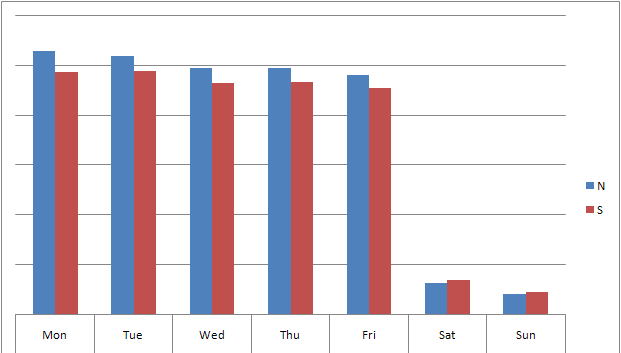
\includegraphics[scale=0.25]{herlev_direction_proportions_morning.png} 
\caption{Herlev - morning}
\label{fig:herlev_props_morning}

    \end{minipage}
    \hspace{0.5cm}
    \begin{minipage}[b]{0.5\linewidth}

\centering
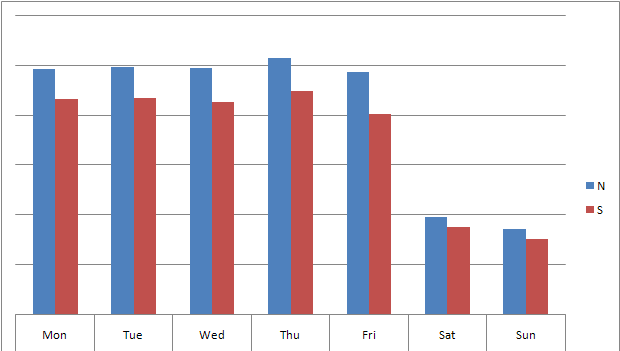
\includegraphics[scale=0.25]{herlev_direction_proportions_afternoon.png} 
\caption{Herlev - afternoon}
\label{fig:herlev_props_afternoon}

    \end{minipage}

\end{figure}

\begin{figure}[ht]

    \begin{minipage}[b]{0.5\linewidth}

\centering
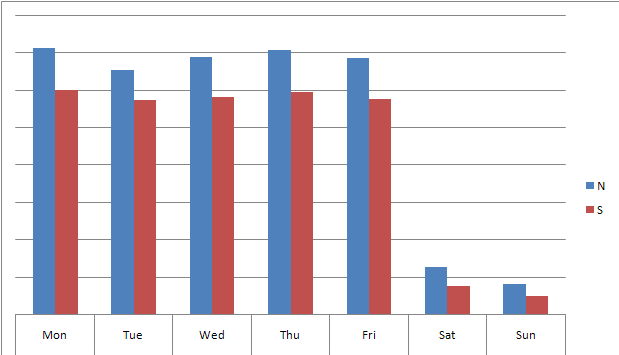
\includegraphics[scale=0.25]{glostrup_direction_proportions_morning.png} 
\caption{Glostrup - morning}
\label{fig:glostrup_props_morning}

    \end{minipage}
    \hspace{0.5cm}
    \begin{minipage}[b]{0.5\linewidth}
    
\centering
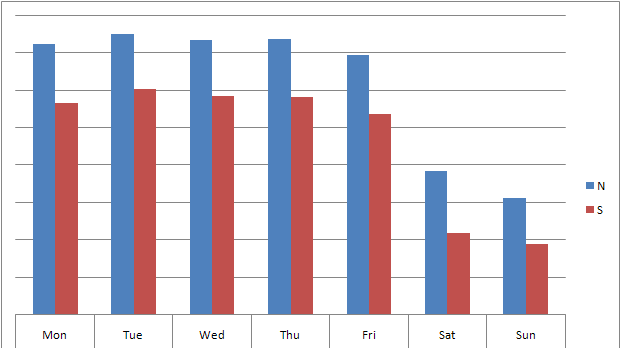
\includegraphics[scale=0.25]{glostrup_direction_proportions_afternoon.png}
\caption{Glostrup - afternoon}
\label{fig:glostrup_props_afternoon}

    \end{minipage}

\end{figure}

We can see that there is an overweight of northgoing traffic. This overweight is more profound in the Glostrup area and increases in the afternoon for both areas.

From these graphs we can also see that, in the weekend, most traffic happens in the afternoon.

The next graph, see Figure \ref{fig:commuter}, shows the usual commuter- and lunch traffic patterns. The data from all mondays to fridays in the dataset have almost identical temporal distributions and thus the graph shows summarized data from workdays.

\begin{figure}[ht]
\centering
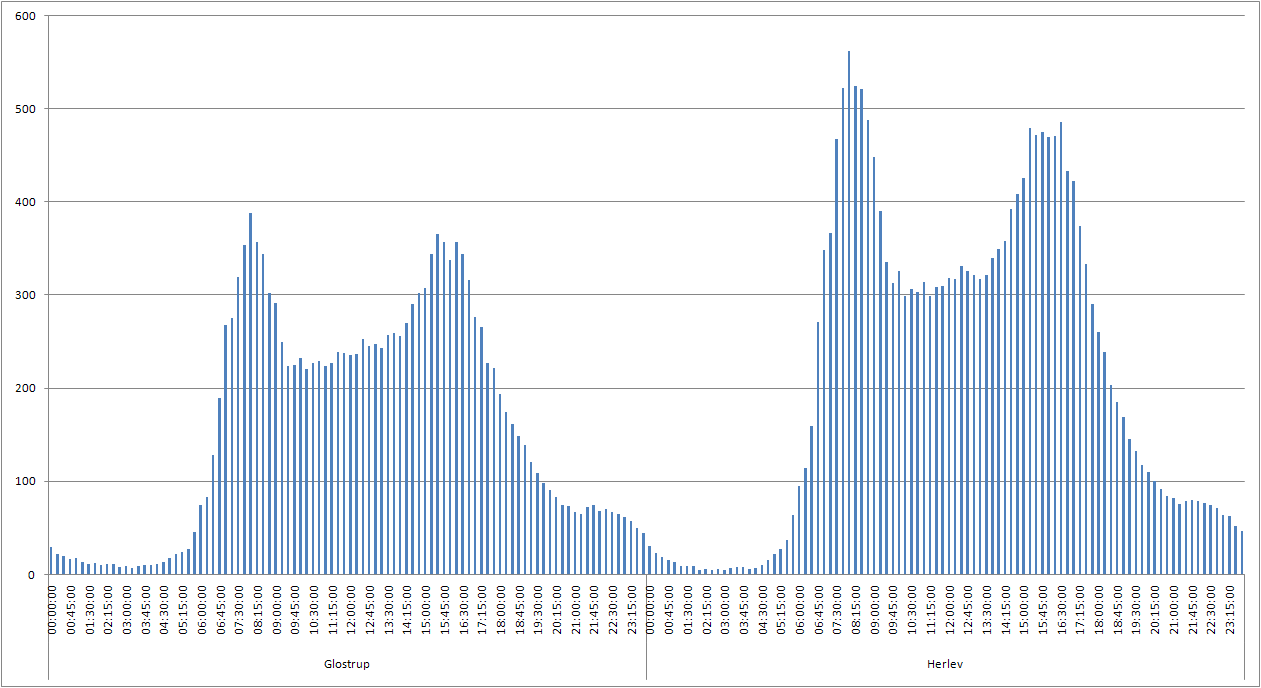
\includegraphics[scale=0.25]{distribution_workday.png} 
\caption{Distribution of traffic throughout workdays in Herlev and Glostrup}
\label{fig:commuter}
\end{figure}

By comparing the workday distribution to the detected traffic in the weekend, see Figure \ref{fig:weekends} - and at the same time looking and the directional proportions - it is clear that ringroad 3 is heavily used by commuters in both Herlev and Glostrup. Traffic is almost identically distributed on saturdays and sundays and the graph shows summarized data for the weekend.

\begin{figure}[ht]
\centering
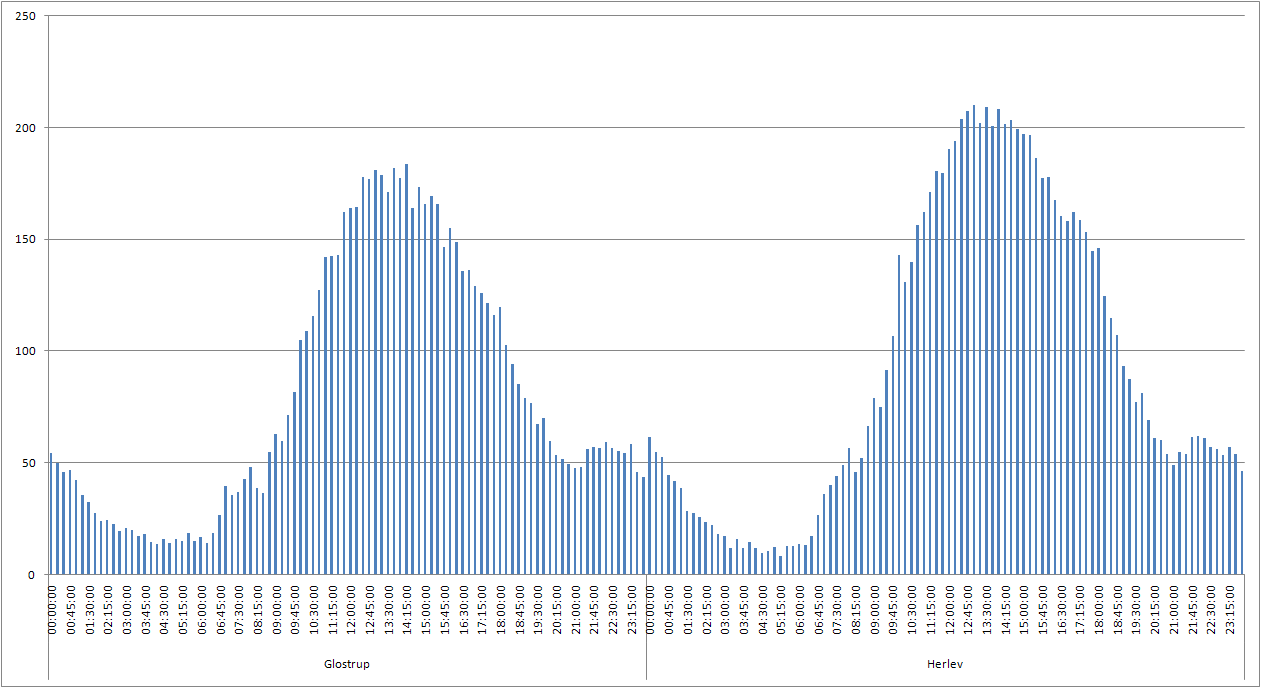
\includegraphics[scale=0.25]{distribution_weekend.png} 
\caption{Distribution of traffic throughout the weekend in Herlev and Glostrup}
\label{fig:weekends}
\end{figure}

The next graph (Figure \ref{fig:detector_directions}) show how detections are aligned in the north and southgoing directions in both areas. (For both directions and areas these proportions do not vary in particular between workday and weekend.)

\begin{figure}[!ht]
\centering
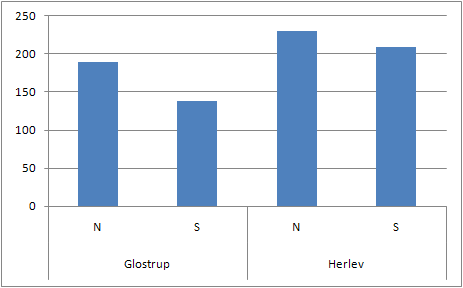
\includegraphics[scale=0.4]{detector_directions.png}
\caption{Relative detections for north- and southgoing links in Herlev and Glostrup}
\label{fig:detector_directions}
\end{figure}

One notable conclusions that can be drawn from these detector data is that there is a slight overweight of traffic north-going traffic in both areas, in the worst case around 3:2, so the direction biased is not profound.

We can also conclude that ringroad 3 in Glostrup and Herlev face heavy commuter traffic by the classical increases in traffic from 7-9 and 15-17 but also from slightly around 12 due to lunch traffic. The background traffic (ie. traffic not directly caused by commuters) through the workdays is heavy as well, starting around 6 and leveling off around 18. Morning and afternoon traffic appears to be quite similar.

\subsection{Traffic Count Analysis}
\label{traffic_count_analysis}

Traffic counts are widely used in traffic planning to setup simulations. They are performed manually by a suitable number of persons, so that each approach and turning motion of an intersection is counted simultaneously.

DRD provided traffic counts for every intersection except Ejby Torvevej (which is a blinded minor road and of little importance according to DRD) which has made it possible to model in detail the turning motions in the network.
The counting period was 7.00-9.00 in the mornings and 15.00-17.00 in the afternoons in 15-minutes intervals. The counts involved, for each approach, the turning movements of cars (including vans) and trucks. 

From table \ref{tab:traffic_counts} we see a listing of the traffic counts and couting dates; most counts are from fall 2001 before the expansion of motorring 3 had begun. It is expected that the traffic has changed since then but the averall changes will probably fluctuate until motorring 3 is finished late 2008 (expected) due to differing conditions over time on motorring 3 (lane closures etc).

For some of the most important intersections (Mileparken, Jyllingevej, Roskildevej) we have newer traffic counts. For Herlev Hovedgade I received a detector count (MASTRA) from 2007 in addition to the traffic count in 2001, however the resolution was 1 hour and there was no distinction between cars and trucks and so it was disregarded.

\begin{table}[!ht]
\centering
\begin{tabular}{l|l|l}
\textbf{\#} & \textbf{Intersection} & \textbf{Date Counted}\\ \hline
1 & Herlev Sygehus & 30-10-2001\\
2 & Hjortespringvej & 09-10-2001\\
3 & Herlev Bygade & 04-10-2001\\
4 & Herlev Hovedgade & 02-10-2001\\
5 & Mileparken & 03-10-2005\\
6 & Ejby Industrivej & 27-02-2001\\
7 & Ejby Torvevej & -\\
8 & Jyllingevej & 23-10-2007\\
9 & Fabriksparken & 04-10-2001\\
10 & Gammel Landevej & 03-10-2001\\
11 & Kindebjergvej & 18-09-2001\\
12 & Roskildevej & 28-08-2003\\
\end{tabular}
\caption{Traffic count dates}
\label{tab:traffic_counts}
\end{table}

The main feat of traffic counts is that the ratio of cars to trucks is available. In Figure \ref{fig:cars2trucks} we see that - in total - there is about the same amount of traffic in each direction, however there are more trucks from south (ie. northgoing) supporting the results on direction bias from the DOGS detector data. Furthermore we are confirmed again on the clear arterial nature of the involved intersections due to the relative volumes of north-south going traffic to traffic from east-west.

The columns E and W indicate the total load of trucks and vehicles coming from east and west respectively, in which we see that the traffic from west, which is travelling towards the city of copenhagen, is somewhat heavier than the traffic coming from east, travelling away from the city.

\begin{figure}[!ht]
\centering
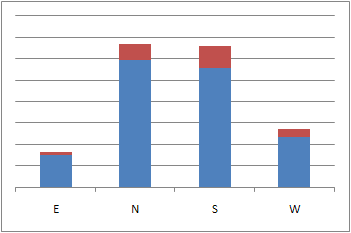
\includegraphics[scale=0.5]{cars_vs_truck_vs_direction.png}
\caption{Combined ratio of cars to trucks from each direction in the morning period. There are more trucks coming from south than from north.}
\label{fig:cars2trucks}
\end{figure}

In Figure \ref{fig:cars2trucks_time} we see how the proportion of cars and trucks evolve over time and note that the proportion remains the same in the sampling period.

\begin{figure}[!ht]
\centering
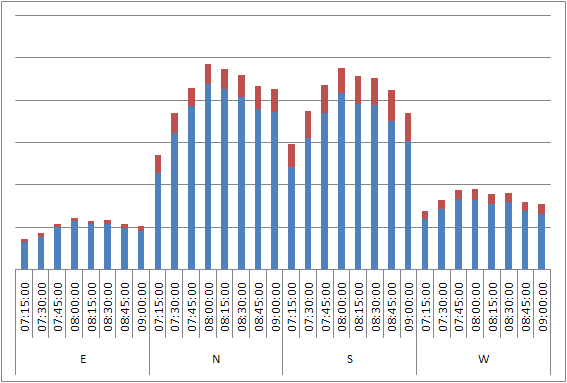
\includegraphics[scale=0.5]{cars_vs_trucks_vs_time_morning.png}
\caption{As Figure \ref{fig:cars2trucks} but over time. The proportion of cars to trucks does not vary much.}
\label{fig:cars2trucks_time}
\end{figure}

In the next figure (\ref{fig:cars2trucks_insect}) we see the proportions of cars to trucks for each intersection. The bars are the sum of cars and trucks in the morning period and also give an indication of the load each intersection faces. We can see that the most heavily loaded intersections are Herlev Hovedgade, Jyllingevej and Roskildevej (disregarding that two latter two were counted later than the other intersections) and that Herlev Hovedgade is the junction which sees the most trucks per car while Jyllingevej serve considerably less trucks. It is interesting to see that these heavily loaded intersections are the ones which were recounted after 2001, except for Mileparken.

\begin{figure}[!ht]
\centering
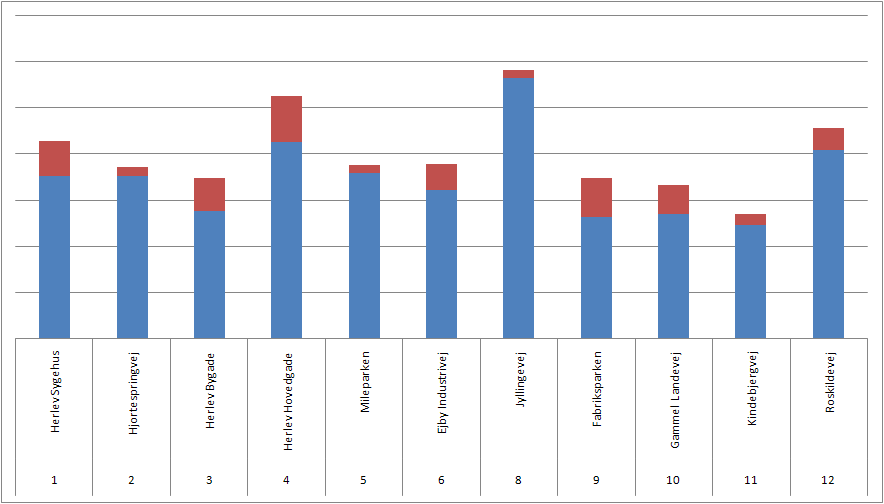
\includegraphics[scale=0.35]{cars_vs_trucks_all_intersections.png}
\caption{Cars to trucks proportions per intersection}
\label{fig:cars2trucks_insect}
\end{figure}

The final two figures (\ref{fig:insect_herlev}-\ref{fig:insect_glostrup}) show, for each DOGS controlled area, the demand faces from each direction split on trucks and cars. 

\begin{figure}[ht]
\centering
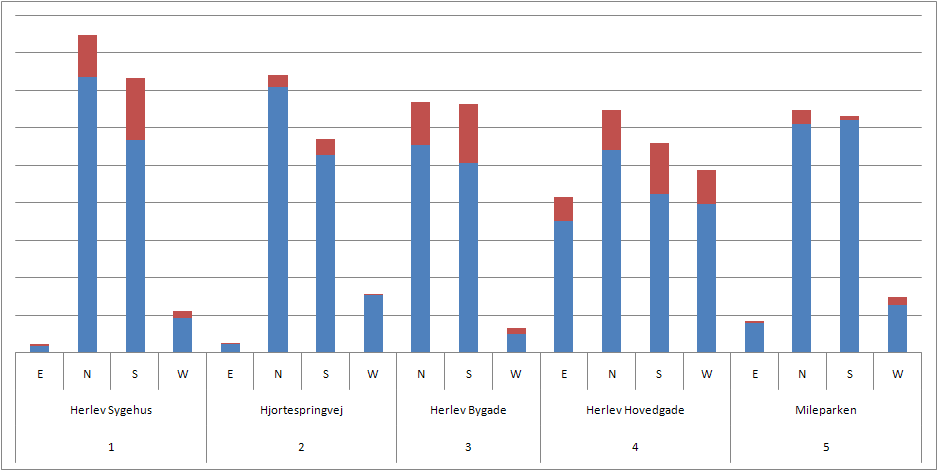
\includegraphics[scale=0.30]{demand_from_direction_per_intersection_herlev.png}
\caption{Demand from direction per vehicle type in Herlev}
\label{fig:insect_herlev}
\end{figure}  
    
\begin{figure}[ht]
\centering
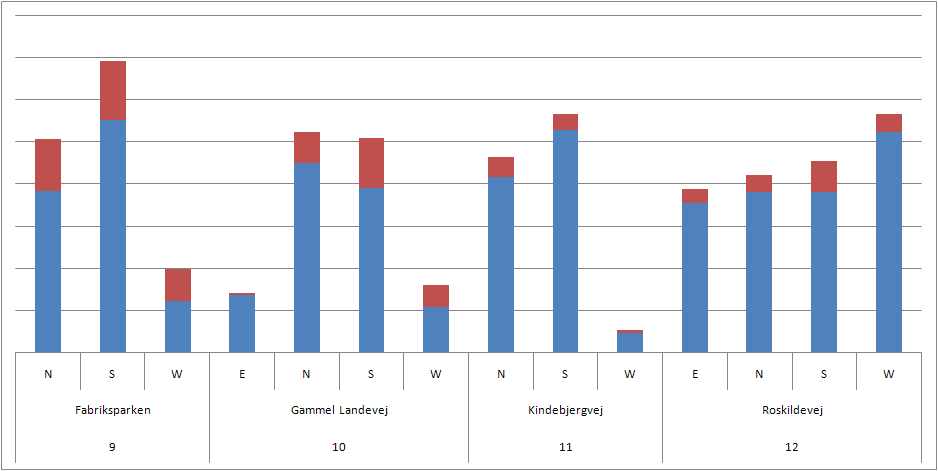
\includegraphics[scale=0.30]{demand_from_direction_per_intersection_glostrup.png}
\caption{Demand from direction per vehicle type in Glostrup}
\label{fig:insect_glostrup}
\end{figure}

In all cases the vehicle demand by far outweighs truck demand; the intersections facing the most truck demand in Herlev are Herlev Hovedgade (from all directions), Herlev Bygade (from north and south) and also Herlev Sygehus from the arterial directions. 

In Glostrup we see that Fabriks has far more northgoing traffic and fair amounts of trucks and both arterial directions. Roskildevej has almost as much traffic from the sideroads as does Herlev Hovedgade, emphasizing the fact that ringroad 3 is not exclusively an artery in the north-south directions for several intersections.
